\chapter{REFERENCIAL TEÓRICO}

    O modelo de referência de redes, o modelo OSI, foi desenvolvido no final dos anos 1970 pela Organização Internacional para Padronização (ISO) para definir a arquitetura das redes de computadores emergentes na época \cite{kurose2014}. A arquitetura é hierárquica e tem por objetivo garantir a independência entre os serviços oferecidos pelas camadas, denominado encapsulamento, sendo que a comunicação entre cada uma das camadas é feita pela adjacente. O modelo OSI é dividido em 7 camadas:
    
    \begin{enumerate}[label=\alph*)]
        \item \textit{layer} 1 - camada física;
        \item \textit{layer} 2 - camada de enlace;
        \item \textit{layer} 3 - camada de rede;
        \item \textit{layer} 4 - camada de transporte;
        \item \textit{layer} 5 - camada de sessão;
        \item \textit{layer} 6 - camada de apresentação;
        \item \textit{layer} 7 - camada de aplicação.
    \end{enumerate}
    
\section{Endereçamento IPv4}
    
    O IPv4 é um protocolo implementado na camada de rede, tendo como objetivo fazer o encaminhamento e o roteamento dos pacotes, tendo como cerne o endereçamento virtual dos dispositivos na rede. Um endereço IP é um identificador único na internet e, para que a unicidade seja garantida, existe um órgão internacional responsável pela administração dos endereços, a IANA, que obedece diretrizes estabelecidas na RFC 2050, delegando blocos de endereços para administração regional, divididos geograficamente nos cinco grupos apresentados na Figura \ref{fig:rir_map}. Na América do Sul, a IANA delega ao LACNIC a administração dos endereços, que por sua vez delega ao NIC.br para controle regional no Brasil, sendo este último órgão recorrido pelos ISPs nacionais para obtenção de blocos de endereços \cite{iana2020}.
    
    \begin{figure}[!htb]
        \centering
        \caption{Mapa global de Regional Internet Registry (RIR) da IANA.} 
        \label{fig:rir_map} 
        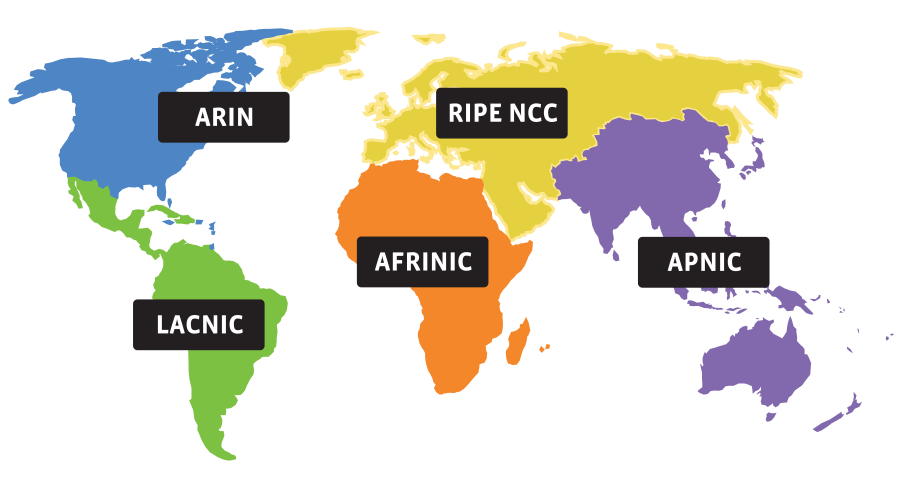
\includegraphics[scale=1.5]{img/rir-map.png} \\
        {\small Fonte: IANA (2020).} 
    \end{figure}
    
\subsection{Cálculos VLSM}

    Um endereço IPv4 é um número de 32 bits, sendo representado na forma \textit{a.b.c.d/x}, em que \textit{x} indica o tamano do prefixo da rede, que representa a quantidade de bits da máscara da rede. Por exemplo, uma máscara 255.255.255.0 é representada por /24. Os $(32 - x)$ bits restantes são os bits dos \textit{hosts}. Essa representação é denominada CIDR, uma representação sem classes, adotada após o endereçamento com classes (A, B, C, D e E) cair em desuso devido ao desperdício na alocação de endereços.
    
    Cálculos de VLSM operam sobre o CIDR e permitem a criação de sub-redes dentro de um sub-rede (recursivamente). Por exemplo, um ISP tem uma rede /21 alocada pelo NIC.br e pode dividi-la em sua intranet em 8 sub-redes /24, ou em 4 sub-redes /23 ou até mesmo em 2 sub-redes /23 mais 4 sub-redes /24 de maneira mista.

\subsection{Mitigando a escassez do IPv4 com NAT}

    O número de dispositivos conectados à internet é crescente e ultrapassa a capacidade de atendimento de IPs que um ISP pode oferer aos seus assinantes. A estratégia adotada é, a princípio, oferer um IP válido na WAN do cliente e uma faixa privada na LAN do mesmo, sendo feita a tradução de endereços na interface WAN/LAN. IPs privados são blocos definidos pela RFC 1918 e não devem ser anunciados na internet, sendo restritos ao uso em intranets para o funcionamento do artifício do NAT.
    
    Existem ISPs que não possuem endereços o suficiente para todos os assinantes, sendo necessário recorrer ao recurso do CGNAT para contornar o problema. O CGNAT implementa uma camada de NAT na WAN do cliente, deixando de entregar um IP válido para alocar um IP privado ao cliente. IPs privados de CGNAT são definidos pela RFC 6598 e são alvos do NAT  operadora, em que um endereço válido é compartilhado por vários assinantes.

\subsubsection{Técnicas de CGNAT}

    Existem duas técnicas adotadas na implantação do CGNAT determinístico, o CGNAT horizontal e o vertical. Ambas garantem a operação do NAT, sendo a diferença entre uma e outra simplesmente a metodologia utilizada no mapeamento entre as redes público-privadas e as faixas de porta.
    
    No modelo horizontal, o mapeamento entre os endereços públicos e privados é feito horizontalmente para uma faixa determinada de portas, como é ilustrado na Figura \ref{fig:cgnat_horizontal}, em que o sentido de crescimento numérico dos endereços privados acompanha os endereços públicos. Essa técnica possibilita a implantação simplificada por uso de ferramentas de \textit{netmapping}.
    
    \begin{figure}[!htb]
        \centering
        \caption{Ilustração do modelo de CGNAT horizontal.} 
        \label{fig:cgnat_horizontal} 
        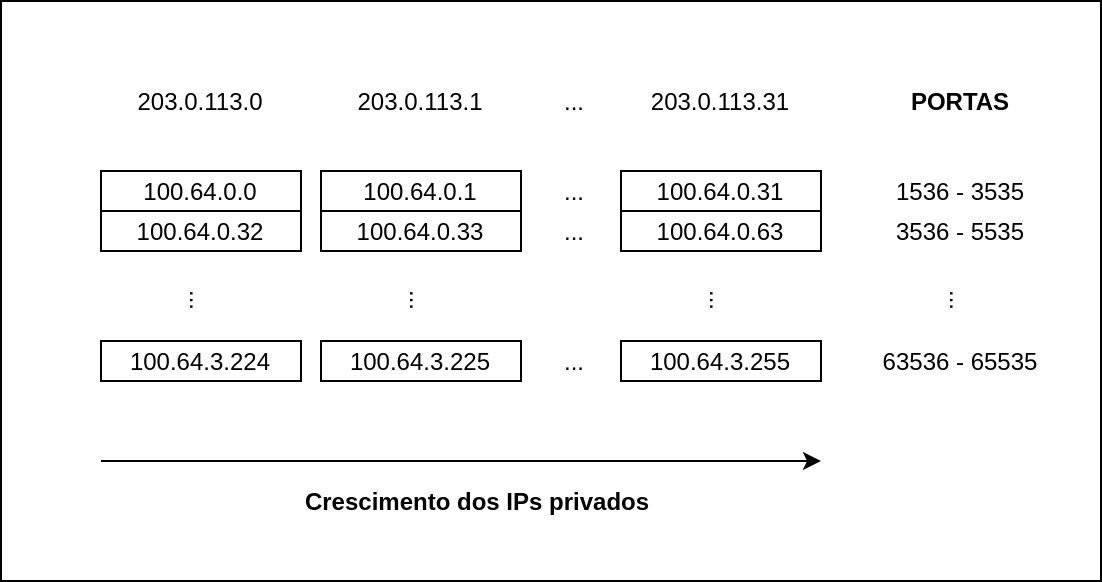
\includegraphics[width=0.9\linewidth]{img/CGNAT-Horizontal.png} \\
        {\small Fonte: do autor (2020).} 
    \end{figure}
    
    No modelo vertical, o sentido de crescimento dos IPs privados não coincide com os IPs públicos, pois o sentido desta vez segue o crescimento do range de portas. Assim, é tomado um IP público como referência e são mapeadas as faixas de portas para os IPs privados consecutivamente, como pode ser visto na Figura \ref{fig:cgnat_vertical}. Essa técnica é de mais fácil entendimento, porém requer mais trabalho para implantação por demandar criação de várias regras individuais de NAT.
    
    \begin{figure}[!htb]
        \centering
        \caption{Ilustração do modelo de CGNAT vertical.} 
        \label{fig:cgnat_vertical} 
        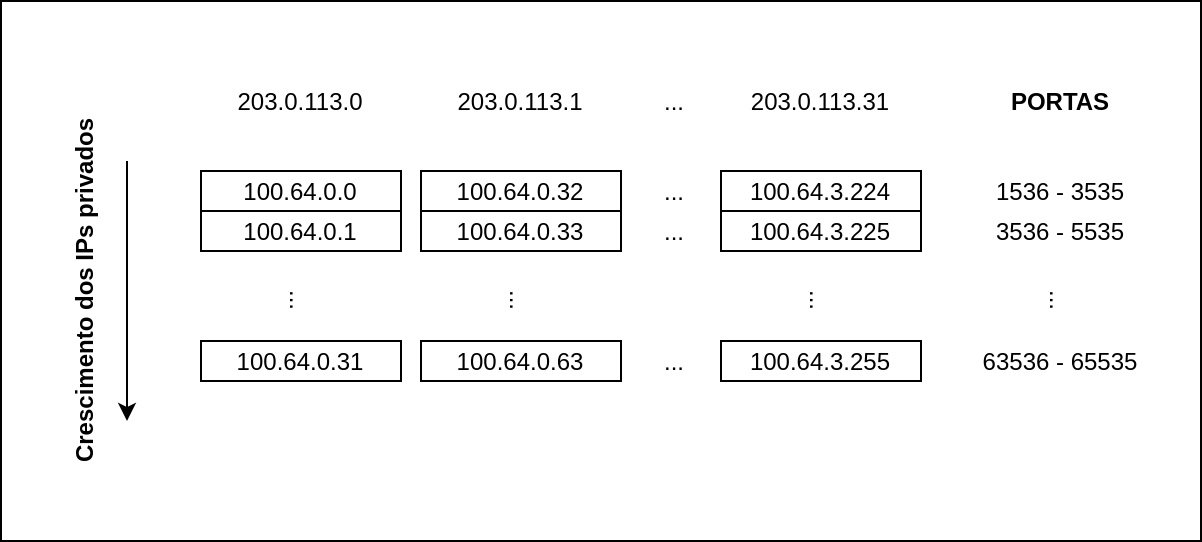
\includegraphics[width=0.9\linewidth]{img/CGNAT-Vertical.png} \\
        {\small Fonte: do autor (2020).} 
    \end{figure}

\subsubsection{Desvantagens do NAT}

    Apesar de solucionar a escassez de endereços de um ISP, o CGNAT implementa uma camada dupla de NAT para os assinantes, o que não permite o funcionamento de redirecionamentos de portas de maneira simples e direta. O redirecionamento de portas nesse cenário, necessita da compatibilidade do dispositivo adotado para implantação do CGNAT e fica limitado a uma faixa de portas definida pelo mapeamento.
    
    Como consequência do NAT duplo, protocolos P2P não funcionam, pois não existe comunicação de entrada direta com o \textit{host}, sendo necessário o uso de recursos para travessia de NAT, como reversão de conexão ou repasses para aplicação com um nó intermediário para resolução da limitação imposta \cite{kurose2014}.
    
    Do ponto de vista do modelo OSI, o NAT viola o encapsulamento da pilha de protocolos por trabalhar em conjunto nas camadas de rede e de transporte, com a tradução entre IP e porta, sem hierarquia. 
    
\subsection{Migração para IPv6}
    
    Como solução aos problemas estruturais e operacionais do NAT, é proposta a migração para o IPv6, que adota como endereço um número de 128 bits, muito mais do que o suficiente para endereçar unicamente todos os dispositivos em LAN sem o uso de IPs privados. Como todos os dispositos tem IP válido com IPv6, não existe o conceito de NAT com o novo protocolo.
    
    Embora o IPv6 seja a solução, não basta apenas o ISP implantá-lo, é necessário que o acordo de tráfego no novo protocolo também esteja fechado com os servidores de sistemas e de provedores de conteúdo. Enquanto isso não seja um tecnologia de ponta-a-ponta, o CGNAT é um modelo satisfatório no processo de transição.

\section{Segurança de ambientes de rede}

    Sistemas em rede estão suscetíveis à ataques, pois a internet é promíscua por sua própria natureza. O objetivo da segurança é minimizar os riscos, pois não existe sistema 100\% seguro, a cada dia são descobertas novas falhas e as correções são constantes.
    
    A segurança da informação é regida por três pilares: confidencialidade, integridade e disponibilidade. A segurança de redes tem seu foco em disponibilidade, prezando pela minimização de fontes de problemas que possam causar inoperabilidade no serviço, seja vinda de falhas físicas até ataques de negação de serviços explorados por vulnerabilidades na rede.

\subsection{Vulnerabilidades que assombram a rede}

    A seguir são citadas algumas das vulnerabilidades de rede que devem ser tratadas através de firewall, extraídas de \cite{nakamura2007}. São configurações simples, mas que caso passem despercebidas, podem ser fonte para exploração de agentes mal intencionados na internet.
    
\subsubsection{Vulnerabilidade de obtenção de informação}
    
    São fontes de informações protocolos como SNMP e NetBIOS, além de banners de protocolos como Telnet e FTP, que aparecem após conexão ao servidor. SNMP e NetBIOS são serviços que devem estar disponíveis apenas para LAN, não fazendo sentido estarem abertos na internet.

\subsubsection{Vulnerabilidade de invasão}

    São portas de entradas para atacantes invadirem o dispositivo, através de ataque de dicionário para adivinhação de senhas por meio protocolos como Telnet, SSH, API e aplicações de gerenciamento, além reconfiguração de equipamentos através de SNMP.

\subsubsection{Vulnerabilidade de negação de serviço}

    São meios de atacantes de DDoS conseguirem amplificar o tráfego e congestionar a rede, explorando protocolos como DNS e SSDP, que têm o pacote de resposta muito maior que a requisição, podendo inundar a rede em um ataque coordenado. SSDP é um serviço de descoberta de LAN e por isso não tem sentido nenhum estar exposto à internet.

\subsection{Firewall}

    Firewall é um ponto entre duas ou mais redes onde é possível controloar todo o tráfego de dados que passa através dele. Assim, esse ponto único constitui um mecanismo utilizado para proteger uma rede confiável de uma rede pública não-confiável \cite{nakamura2007}.
    
    As técnicas básicas de firewall são a filtragem de pacotes estática (\textit{stateless}) e a filtragem de pacotes baseada em estados (\textit{stateful}). No firewall \textit{stateless}, as regras são aplicadas na camada de rede (camada 3) e de transporte (camada 4), sendo feita a filtragem a partir das informações de IP, porta e protocolo contidas no cabeçalho do pacote, apresentando alto desempenho e performance para gerenciamento de tráfego devido a sua simplicidade. Em contrapartida, não é uma técnica suficiente para filtragem de serviços de portas dinâmicas, o que é possível de ser tratado com um firewall \textit{stateful}, que mantém registros das conexões para filtragens mais inteligentes e dinâmicas, tendo como custo um maior consumo de recursos de processamento.
    
    O firewall não é a solução total para segurança da rede. Selecionar os usuários que podem acessar a rede e definir os direitos que têm na rede, além de determinar os recursos que cada usuário em particular pode acessar e os níveis de acesso são fundamentais. A autenticação e a autorização são também importantes aspectos a serem implementados na infraestrutura de segurança \cite{nakamura2007}.

\subsection{VPN}

    Uma VPN tem como funcionalidade prover conexão a uma rede local através da internet por meio de um túnel de conexão, provendo serviço de acesso remoto como também servindo de mecanismo para controle de acesso, fornecendo uma camada de autenticação à rede interna e autorização quando combinada com um firewall.
    
    Os conceitos que fundamentam a VPN são a criptografia e o tunelamento. A criptografia é utilizada para garantir a autenticidade, o sigilo e a integridade das conexões, e é a base da segurança dos túneis VPN \cite{nakamura2007}. Uma VPN implantada com protocolo PPTP ou L2TP garantem somente autenticidade, enquanto IPSec e protocolos baseados em TLS (como Stunnel e aplicações modernas de VPN) somam integridade e confidencialidade ao túnel.

\section{Topologia de um ISP}
    O modelo comum de topologia adotado por operadoras de internet é formado por um triângulo entre roteadores B-RAS, CGNAT e borda, conforme Figura \ref{fig:isp}. Os clientes finais conectam-se a rede através de PPPoE ao roteador B-RAS, que por sua vez encaminha o tráfego de IP público à borda que será roteada para a internet. Tráfego intermediário de CGNAT (RFC 6598) é encaminhado ao equipamento que traduz os IPs privados em públicos antes de serem roteados à internet.
    
    Dependendo da dimensão da rede, é possível adotar modelos simplificados para economia de recursos, fazendo a mescla das funções de um ou de mais equipamentos em um único só, desde que o equipamento suporte essa configuração.
    
    \begin{figure}[!htb]
        \centering
        \caption{Modelo de topologia de um ISP.} 
        \label{fig:isp} 
        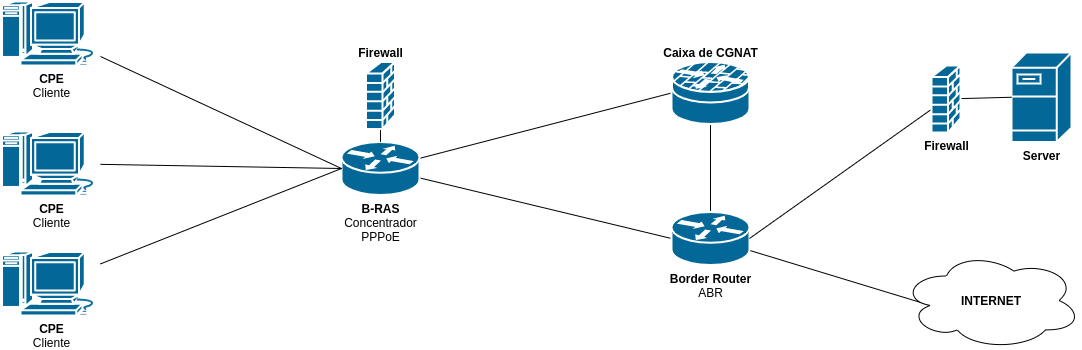
\includegraphics[width=0.9\linewidth]{img/isp.png} \\
        {\small Fonte: do autor (2020).} 
    \end{figure}
    
    Na infraestrutura lógica do ISP também entra os servidores de serviços locais, que provém servidores de autenticação RADIUS, serviço de DNS locais para respostas mais rápidas, Proxy HTTP (CDN) para poupar consumo de banda de internet e serviço de VPN.